Traditional character recognition technology is widely applied to such problems as converting scanned books to text and converting images of bank checks into valid payments. These problems can be divided into offline and online recognition.
We introduce a new problem: identifying characters in a stream of 3d points from fingers. Many OCR techniques utilize images of completed words, whereas this paper deals with interpreting the data as it is generated, specifically for the scenario of writing "in the air."  
This paper deals with online character recognition. With new innovations in computer vision, precise 3D finger data can be obtained at over 100 frames per second, so this paper also proposes a method of doing online character recognition, using a data-driven approach. We can treat the input data from the computer vision device as a multivariate time series.
\marginpar{
\begin{figure}
  \begin{center}
  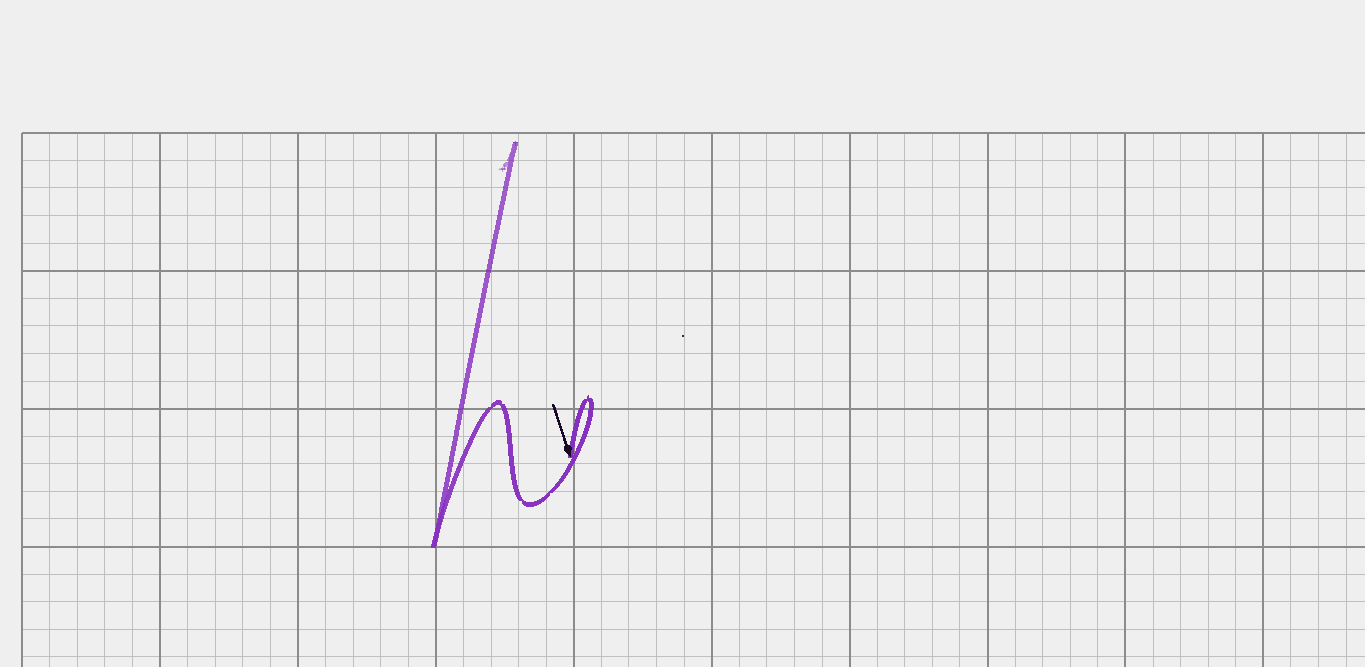
\includegraphics[width=1.75in]{images/he-2d-white.PNG}
  \caption{A 2D view of LEAP data}
  \label{fig:teaser}
  \end{center}  
\end{figure}
}
The task of identifying characters in a time series requires data to test on. Therefore, a new dataset needs to be created, partitioned into candidate time series, specifically the characters in the alphabet, and testing time series, which are words that to be recognized. To construct this dataset, the LEAP Motion, a commercial computer vision device, will be used to record and store data. The experiment will consist collecting the same data from  (insert number) people to account for differences in handwriting.
The proposed approach to identify characters in these time series uses the dynamic time warping (DTW) algorithm. A series of recent optimizations make a real time DTW similarity search feasible in real time. This paper benchmarks the performance of such a similarity search with the given application of handwriting recognition.
The applications of such a technique would be a replacement for the keyboard and mouse altogether. Users can user their computer as normal by moving their finger along with the mouse. When a text input is selected by the mouse, the handwriting input mode would be used, and the stream of finger data points would be interpreted as letters and be sent as input to the computer.
